\documentclass[10pt,a4paper]{article}
\usepackage[utf8]{inputenc}
\usepackage[italian]{babel}
\usepackage{amsmath}
\usepackage{amsfonts}
\usepackage{amssymb}
\usepackage{graphicx}
\usepackage{gensymb}
\usepackage[left=2cm,right=2cm,top=2cm,bottom=2cm]{geometry}
\newcommand{\rem}[1]{[\emph{#1}]}

\author{Gruppo BN \\ Federico Belliardo, Marco Costa, Lisa Bedini}
\title{Esperienza 10: caratteristiche fisiche porte logiche}

\begin{document}
\maketitle

\section{Scopo dell'esperienza}
Lo scopo dell'esperienza è misurare le caratteristiche statiche e dinamiche delle porte NOT dell'integrato SN74LS04.

\section{Materiale occorrente}
\begin{itemize}
\item IC SN74LS04;
\item trimmer da 2 k$\Omega$ 10 k$\Omega$ e 100 k$\Omega$;
\item Arduino Nano;
\item IC SN74LS244;
\end{itemize}

\section{Caratteristiche statiche}
Abbiamo montato il circuito come in figura \ref{fig:circuito}.
\begin{figure}
\centering
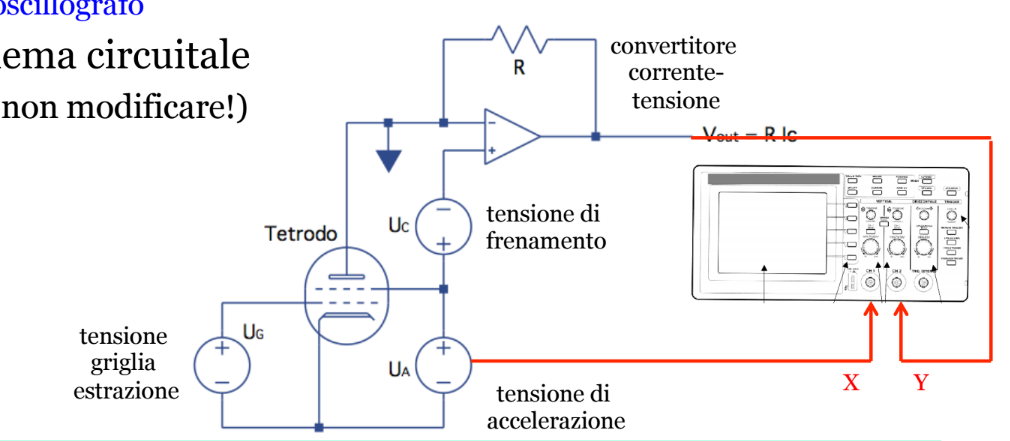
\includegraphics[scale=0.7]{circuito.png}
\caption{Circuito utilizzato.\label{fig:circuito}}
\end{figure}
I valori delle componenti sono state misurate tramite multimetro digitale. Come incertezze abbiamo preso quelle riportate sul manuale dello strumento.
Abbiamo misurato la tensione di alimentazione $V_{CC}=4.85\pm 0.03$V tramite multimetro digitale (incertezza riportata nel manuale), nei limiti di funzionamento riportati nel datasheet.
%R_trimmer totale = 1950.
%R_1=99.6 ohm
\subsection{Misura delle tensioni di operazione}
Per ottenere diversi valori di $V_{in}$ abbiamo variato opportunamente il trimmer (che ha la funzione di partitore di tensione). Una volta fissata la sua posizione, abbiamo misurato tramite multimetro digitale\footnote{E' lo strumento di misure di tensione in continua con maggiore resistenza interna.} $V_{in}$ e $V_{out}$.
In tabella \ref{tab:vinvout} e in figura \ref{fig:vinvout} abbiamo riportato le misure ottenute.
\begin{figure}
\centering
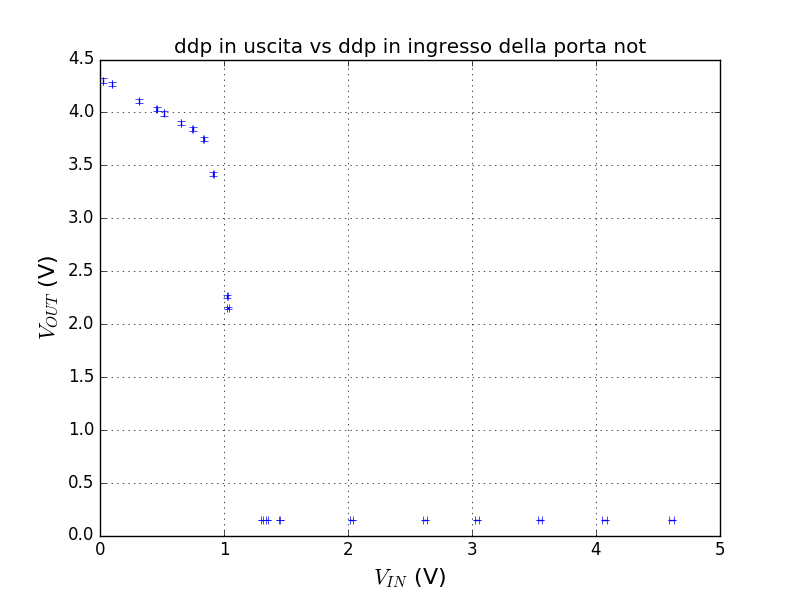
\includegraphics[scale=0.9]{vinvout.png}
\caption{$V_{out}$ in funzione di $V_{in}$.\label{fig:vinvout}}
\end{figure}

\begin{table}
\centering
\begin{tabular}{|c|c|}
\hline
0 & 0\\
\hline
\end{tabular}
\caption{Misure dei potenziali $V_{in}$, $V_{out}$.\label{tab:vinvout}}
\end{table}
%Con i dati abbiamo dato una stima dei valori dei potenziali di input/output a livello alto e basso, riportati in tabella \ref{tab:stime}.
Si osserva che $V_{out}$ va da un massimo di $V_{OH,max}=4.3 \pm 0.1$V fino a 
%sicuro di questa definizione? 
$V_{OH,min}=3.7\pm 0.1$V, valore subito dopo il quale si osserva una rapida variazione di $V_{out}$, dopo la quale si ha transizione al livello basso dell'Otput. %\footnote{In effetti se immaginiamo di tracciare due rette per i due regimi, l'intersezione fra queste due dà un valore vicino a 3.7.}. 
Come incertezza si è preso il range in cui si distinguono i due regimi.
Si può considerare quindi che l'uscita della porta sia al livello alto nella fascia trovata. Pertanto abbiamo stimato $V_{OH}=3.7\pm0.2$V\footnote{In accordo con la definizione data di $V_{OH}$.}. Abbiamo stimato l'incertezza su questo valore come la differenza fra il primo punto per cui si è osservata la variazione e quello immediatamente precedente.

Come stima di $V_{OL}$ abbiamo preso $0.15 \pm 0.05$V, ossia il valore asintotico. Abbiamo tuttavia una grande incertezza su questa stima: in effetti abbiamo riscontrato difficoltà a prendere misure per valori di $V_{out}$ poco superiori a $0.144$V; in particolare, era sufficiente una leggera variazione della posizione del trimmer per portare $V_{out}$ dal valore di $2.15$V a $0.144$V.
Per quanto riguarda le tensioni in ingresso, si osserva che esse vengono considerate dalla porta come valore basso in un range che va da $0$ a $0.8$V circa, mentre alto da $1.3$V in poi.
Per stimare i valori di soglia $V_{IL}$, $V_{IH}$, abbiamo preso i valori di $V_{in}$ per i quali si osserva l'inizio della transizione di $V_{out}$ da un livello logico all'altro. Con i dati presi si è stimato $V_{IL} = 0.8\pm 0.1$V, dove come incertezza abbiamo preso la differenza di $V_{IL}$ dal primo valore di $V_{in}$ per il quale $V_{out}$ inizia a scendere bruscamente.
In modo del tutto analogo si ha $V_{IH} = 1.3\ pm 0.2$V. 
I valori stimati risultano tutti in buon accordo con quanto riportato sul datasheet:
$V_{IL,att}= 0.8$V, $V_{IH, att}=2$V, $V_{OL, att}=0.25$V, $V_{OH, att}=3.4$V.
Il comportamento che si osserva per valori di $V_{in}$ compresi fra $V_{IL}$ e $V_{IH}$ può essere spiegato in termini del circuito in figura \ref{fig:ttl}.

\begin{figure}
\centering
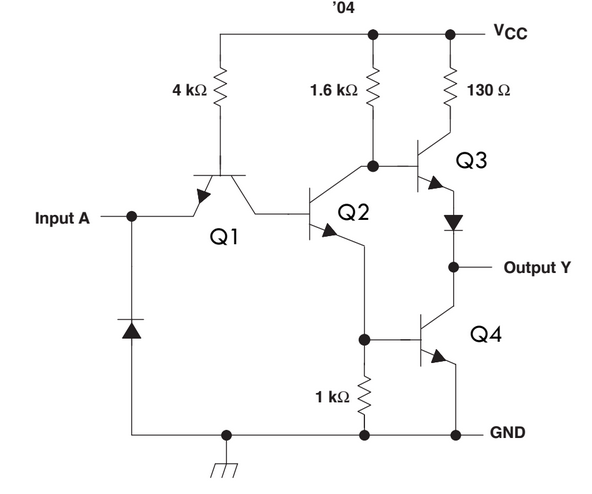
\includegraphics[scale=0.6]{ttl.png}
\caption{Schema circuitale di NOT TTL (presente negli '04).\label{fig:ttl}}
\end{figure}

Quando si supera $V_{IL}$ (ossia si passa da stato basso a alto), il transistor Q1 passa dal regime di saturazione a interdizione; conseguentemente Q2 e Q4 passano da regime di interdizione a saturazione (scorre corrente nella maglia che non contiene Q1) e l'output cambia stato. Dato che le transizioni nei transistor non sono immediate, ed è necessario che le varie giunzioni cambino polarità, si ha una fascia di $V_{in}$ compresa tra $V_{IL}$ e $V_{IH}$ in cui si ha un $V_{out}$ intermedio fra $V_{OH}$ e $V_{OL}$.
 
%manca spiegazione teorica dell'andamento di transizione
\subsection{Misura delle correnti in ingresso}
Abbiamo inserito l'amperometro in serie all'ingresso del circuito di figura \ref{fig:circuito} e abbiamo misurato $I_{in}$ al variare di $V_{in}$\footnote{La procedura per variare $V_{in}$ è la stessa del punto precedente.}. Per avere più sensibilità sulla misura di corrente si è usato il multimetro analogico e l'incertezza usata è quella riportata nel manuale. Il segno di $I_{in}$ è positivo se entrante nella porta.
%Qua ci va una breve discussio teorica sul verso della corrente e l'andamento)
I dati sono riportati in tabella\ref{tab:viniin} e in figura \ref{fig:viniin}.
\begin{figure}[!htb]
\centering
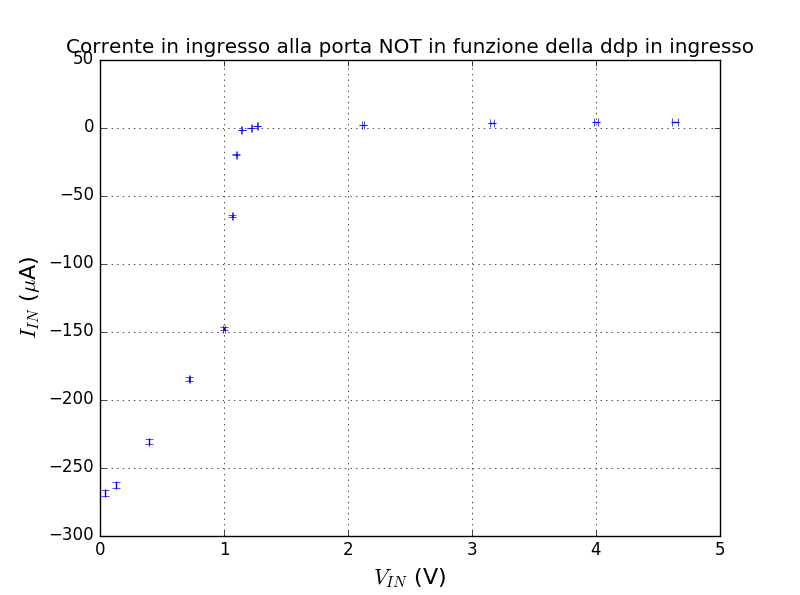
\includegraphics[scale=0.9]{viniin.png}
\caption{Corrente in ingresso alla porta NOT in funzione di $V_{in}$.\label{fig:viniin}}
\end{figure}
Ci aspettiamo che per $V_{in}$ a livello basso si abbia una corrente uscente (negativa), in quanto l'input è come se fosse collegato direttamente a $V_{CC}$ tramite la giunzione polarizzata direttamente BE di Q1 ( figura \ref{fig:ttl}). Viceversa, se $V_{in}$ è alto, Q1 è in interdizione e quindi si avrà una corrente entrante circa nulla.
Si osserva che per $V_{in}$ corrispondenti al valore logico basso, si ha una corrente $I_{in}$ negativa e dell'ordine delle centinaia di $\mu \mbox{A}$ (massimo sui $260\mu \mbox{A}$), mentre per $V_{in}$ su stato alto, si ha una corrente nulla entro l'errore.
Abbiamo stimato i valori delle correnti di soglia in corrispondenza dei punti in cui si hanno variazioni brusche dell'andamento di $I_{in}$\footnote{Questi sono anche punti in cui $V_{in}$ è prossimo a $V_{IL}$, $V_{IH}$.}.
Si ha quindi $I_{IH}=0.0\pm0.5\mu \mbox{A}$ e $I_{IL}=-180\pm20\mu\mbox{A}$
I rispettivi valori massimi riportati sul datasheet sono $I_{IL,att}=-0.4\mbox{mA}$, $I_{IH}=20\mu\mbox{A}$. 
% frase ripetuta? I valori riportati nel datasheet sono $I_{IL,att}=-0.4\mbox{mA}$, $I_{IH,att}=\mu \mbox{A}$
I valori stimati quindi rientrano nei limiti riportati dal costruttore. 
%sei sicuro di questa definizione delle correnti??
%Confronto coi valori del datasheet
\subsection{Misura delle correnti in uscita}
Per misurare la massima e minima corrente in uscita dalla porta, abbiamo montato il circuito \footnote{Il circuito collegato all'ingresso della porta è lo stesso di prima.} come in figura \ref{fig:circuito2}. Per ricavare $I_{out}$ abbiamo misurato la caduta di potenziale $V_{AB}=V_A-V_B$ ai capi della resistenza $R_2$ tramite multimetro digitale e poi si è diviso per $R_2=98\pm 1 \Omega$. Si è preso il segno della corrente positivo se entrante nella porta.
\begin{figure}
\centering
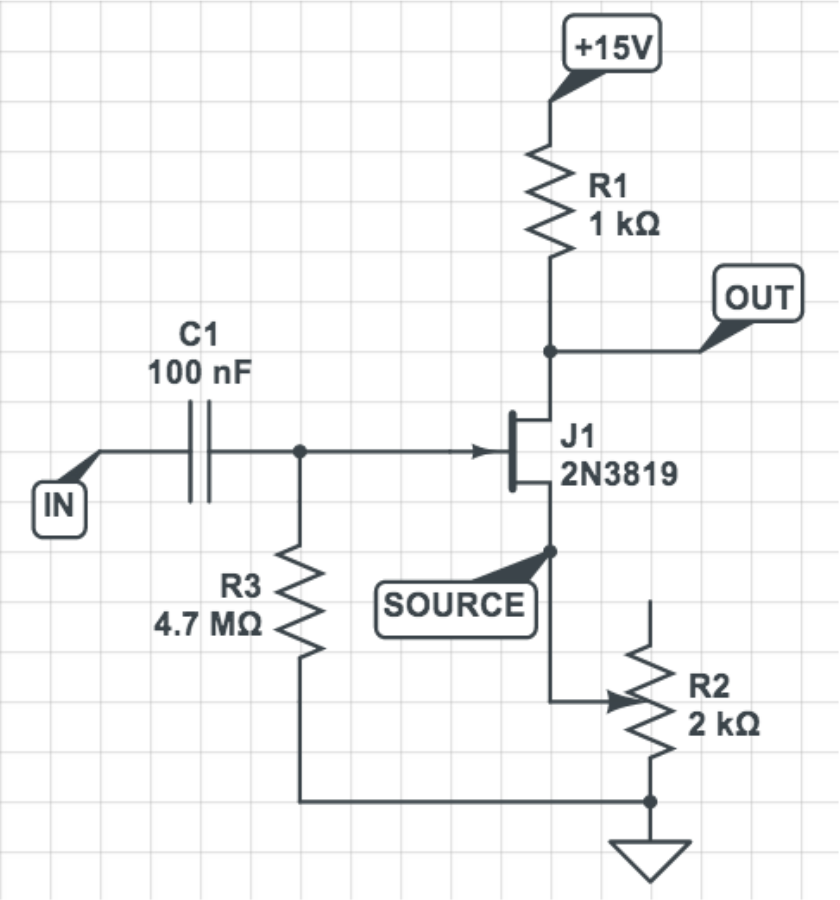
\includegraphics[scale=0.7]{circuito2.png}
\caption{Schema del circuito utilizzato per la misura delle correnti di uscita.\label{fig:circuito2}}
\end{figure}
Per la misura di $I_{OL}$ si collega l'uscita a $V_{CC}$  e si varia il potenziometro $R_1$ in figura \ref{fig:circuito2} in modo che l'uscita sia in stato basso.
Per verificare che l'uscita fosse effettivamente nello stato basso, si è controllato $V_{out}$ tramite oscilloscopio. Abbiamo deciso di prendere la misura di corrente in corrispondenza del valore di $V_{OL}$ stimato in precedenza. Tuttavia, in questo modo si ottiene $V_{AB}=4.60\pm 0.4$mV e quindi $I_{out}=47\pm 1 \mu \mbox{A}$, che risulta più basso del valore riportato sul datasheet $I_{OL,att}=8$mA. Abbiamo quindi deciso di prendere una ulteriore misura, in corrispondenza del punto in cui si osservava una brusca variazione di $V_{out}$ e $V_{AB}$. Ciò avviene per $V_{out}=380\pm3$mV e $V_{AB}=700\pm7$ mV, da cui $I_{out}=7.1\pm 1$mA. 
Così si ottiene una stima più vicina al valore nominale. Abbiamo quindi scelto questo valore come $I_{OL}$. Un motivo per cui fallisce il metodo di stimare $I_{OL}$ come la $I_{out}$ a $V_{OL}$ è che nelle misure riportate nel grafico \ref{fig:vinvout} non si è riusciti a ottenere misure di $V_{out}$ che non fossero del valore limite $0.144$V. In effetti, sempre facendo riferimento allo stesso grafico, si osserva che il $V_{out}$ a cui è stata presa $I_{OL}$ non è così lontano dalla zona in cui l'output è considerato basso.
Per la misura di $I_{OH}$ si collega l'uscita al ground facendo in modo che essa sia in stato alto.
Abbiamo preso la misura in corrispondenza di $V_{OUT}=3.7\pm0.1 $V, ossia il valore stimato di $V_{OH}$ (in corrispondenza di tale valore si aveva anche una brusca variazione della corrente e di $V_{OUT}$).
Così si ottiene $V_{AB}=-13.8$mV e quindi $I_{OH}=-0.141\pm0.001$mA, valore in accordo con quanto riportato nel datasheet $I_{OH,att}=-0.4$mA. La strategia di mettere $V_{out}$ pari alla stima del valore di soglia ottenuto in questo caso funziona meglio perchè i dati del grafico \ref{fig:vinvout} coprono un intorno sufficientemente grande del punto in cui avviene la variazione brusca di corrente.
Una spiegazione della rapida variazione di $I_{in}$ è che se diminuiamo troppo la resistenza di carico all'uscita della porta NOT, l'integrato deve erogare più corrente affinchè ci sia la giusta differenza di potenziale fra $V_{out}$ e $V_{A}$ (il quale è tenuto a potenziale costante tramite opportuno collegamento). Se la corrente necessaria supera la corrente massima erogabile, il circuito non funziona più come NOT e quindi si ha una variazione della corrente.  
%discussione teorica andamento
Con questi valori si è dato una stima del \emph{fanout}.
Le correnti che determinano tale valore sono $I_{OL}$ e $I_{IL}$, in quanto $I_{IH}$ è nulla (al più dell'ordine del $\mu$A), e quindi si possono alimentare più facilmente porte quando si è nello stato alto.
Si ha $\emph{fanout}= I_{IL}/I_{OL}=39\pm 2$, mentre utilizzando le correnti di soglia nominali si ottiene $\emph{fanout, att}=20$. Il risultato ottenuto è dello stesso ordine di grandezza di quello stimato.
\section{Montaggio di Arduino}
%R_1=0.98k
%R_2 = 1.003 k 
%R_3 = 0.976 k
%R_4 = 0.989 k
%R_5 = 9.94 k
%C_2 = 106.5 nF
%C_1 = 106.6 nF
Abbiamo montato il circuito pulsatore in figura \ref{fig:arduino}.
\begin{figure}
\centering
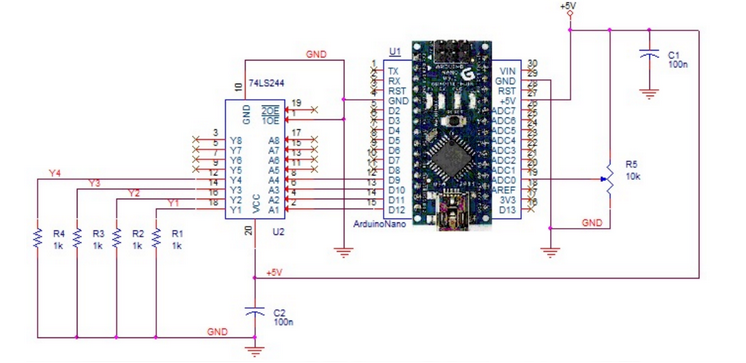
\includegraphics[scale=0.7]{arduino.png}
\caption{Schema del pulsatore utilizzato.\label{fig:arduino}}
\end{figure}
Successivamente abbiamo verificato il suo comportamento da generatore di onde quadre. La frequenza del segnale dipende dalla posizione del trimmer, e va da qualche Hz ai 50 kHz. L'ampiezza dell'onda picco-picco è pari a $v_{pp}=3.16\pm 0.04$V.
\begin{figure}
\centering
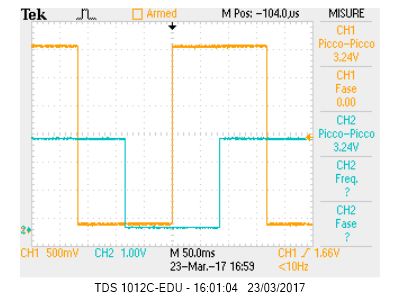
\includegraphics[scale=0.7]{ondaardu.png}
\caption{Onde sfasate di $\pi/2$ in uscita a $Y_1$, $Y_2$. L'ampiezza dei segnali è la stessa, si sono solo usate scale diverse per comodità grafica.\label{fig:ondaardu}}
\end{figure}
In figura \ref{fig:ondaardu} si possono osservare i segnali (misurati tramite oscilloscopio) alle uscite $Y_1$ e $Y_2$.
\section{Caratteristiche dinamiche}
\subsection{Onda in ingresso}
Si è generato tramite Arduino un segnale ad onda quadra di frequenza di circa $1.01\pm0.01$kHZ di ampiezza da 0 a $3.16\pm 0.04$V.
In figura \ref{fig:ondanot} si può osservare il corretto funzionamento della porta NOT.
\begin{figure}
\centering
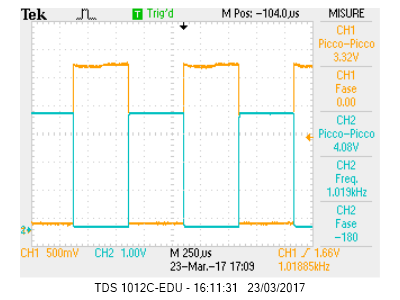
\includegraphics[scale=0.7]{ondanot.png}
\caption{\label{fig:ondanot}}
\end{figure}
Si è effettuata la misura tramite oscilloscopio. Le incertezze sui potenziali sono la sensibilità del cursore più il $3\%$ di calibrazione, mentre sui tempi il massimo fra la sensibilità del cursore e la semidispersione dei valori plausibili.

\subsection{Misura dei tempi di propagazione}
Abbiamo eseguito una misura dei due tempi di propagazione, misurando il tempo fra i segnali in ingresso e in uscita in corrispondenza dei i due punti a metà altezza della rampa in salita (tPLH) e discesa (tPHL) rispettivamente.
In figura \ref{fig:tphl} e \ref{fig:tlph} si possono osservare il tempo di propagazione $tPHL$ e $tPLH$ rispettivamente.
\begin{figure}
\centering
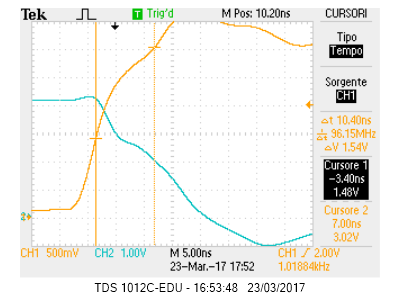
\includegraphics[scale=0.6]{tphl(meglio).png}
\caption{Tempo di propagazione $tPHL$.\label{fig:tphl}}
\end{figure}

\begin{figure}
\centering
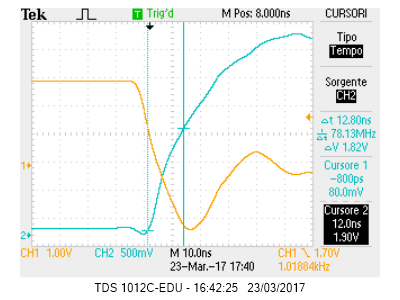
\includegraphics[scale=0.6]{tplh.png}
\caption{Tempo di propagazione $tPLH$.\label{fig:tplh}}
\end{figure}
La misura di tempo è stata eseguita tramite oscilloscopio. L'incertezza sui tempi è dovuta sia alla sensibilità dei cursori, sia all'incertezza sul trovare i punti con il giusto pontenziale. Per stimarla si è presa la semidispersione sui valori misurati nei punti con potenziale compatibile con la metà entro la sensibilità del cursore dei potenziali\footnote{L'oscilloscopio utilizzato consentiva di visualizzare contemporaneamente entrambe le coordinate del punto in cui si prendeva la misura.}.
I valori riportati nel datasheet sono
$tPHL_{att}=10 \mbox{ns}$ e $tPLH_{att}= 9\mbox{ns}$\footnote{Valori tipici con resistenza di carico $R_L = 2\mbox{k}\Omega$.}. 
I valori misurati sono $\mbox{tPHL} = 10.2\pm0.2$ns  e $\mbox{tPLH} = 12.8\pm0.4$ns, pertanto sono in buon accordo con quanto riportato dal costruttore.

%tPHL = 13.20 \pm 0.4 ns seconda: 10.2\pm 0.4 ns
%tPLH = 12.8 pm 0.4ns
%riesci a dare motivazioni teoriche??
\subsection{Misura del tempo di salita}
Abbiamo misurato i tempi di salita $t_{s}$ e discesa $t_{d}$ del segnale in uscita e in ingresso, ossia il tempo necessario per passare dal $10\%$ della $v_{pp}$ massima\footnote{Ai fini dei calcoli si considera $v_{pp}$ senza overshoot.} al $90\%$ (il contrario per il tempo di discesa).
In figura \ref{fig:tsalitain} abbiamo riportato il tempo di salita del segnale in ingresso per mostrare la procedura di misura utilizzata.
\begin{figure}
\centering
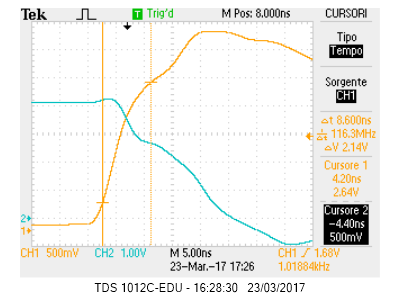
\includegraphics[scale=0.6]{tsalitain.png}
\caption{Tempo di salita del segnale in ingresso.\label{fig:tsalitain}}
\end{figure}

In tabella \ref{tab:tempisalita} sono riportati le misure:
\begin{table}
\centering
\begin{tabular}{|c|c|c|}
\hline
Segnale & $t_{s}$ (ns) & $t_{d}$ (ns) \\
\hline
Ingresso & $8.6 \pm 0.2$  & $6.0 \pm 0.2$  \\
\hline
Uscita & $36.2\pm 0.2$ &  $20.4\pm0.4$    \\
\hline

\end{tabular}
\caption{Tempi di salita e discesa all'ingresso e all'uscita della porta NOT.\label{tab:tempisalita}}
\end{table}
%t_s, in = $8.6 \pm 0.2$ ns
%t_d, in = $6.0 \pm 0.2$ ns
%t_s, out = $36.2\pm 0.2$ ns
%t_d, out = $20.4\pm0.4$ ns
%spiegare discrepanze nel circuito grazie a schema circuitale
\section{Conclusioni}
L'integrato si comporta come porta NOT entro i potenziali indicati dal costruttore. La stima delle correnti di soglia in uscita $I_{OL}$, $I_{OH}$ ha riportato alcune difficoltà, e i valori non sono in completo accordo con quanto riportato sul datasheet.
Il comportamento dinamico del circuito presenta ritardi nella propagazione del segnale in uscita.

\end{document}
